% !TeX root = Report.tex
\section{Introduction}

\subsection{What is a Wireless Sensor Network?}

A wireless sensor network, or WSN for short, is a collection of computing devices called motes; these motes are capable of short range wireless communication and they have the ability to sense their surrounding environment \cite{Mica2002}. The network forms a distributed system that can perform a variety of distributed algorithms, usually data gathering and similar tasks. To communicate, each node is equipped with a radio that allows it to send and receive messages to neighbouring nodes within a limited range. To sense the environment motes typically have a range of embedded sensors such as heat, light, humidity and many others. They also contain a simple central processing unit (CPU), which is programmed to control the hardware on the motes. The CPU also processes events which are triggered by the hardware (such as messages being sent and received) and it also handles any other computation necessary for the operation of the system. As the platform is wireless the motes do not operate on a mains power supply, instead they are powered by energy stored in a battery. Wireless sensor networks as a platform have a wide range of practical applications that stretch from battlefield intelligence for the military \cite{Akyildiz2002393,1368897,1457970} to industrial process monitoring for manufacturing companies \cite{1219475,4796311,4109116}.

A defining characteristic of designing applications for wireless sensor networks is the restricted and finite energy supply available to each node. Therefore, wireless sensor nodes tend not to use expensive broadcasting protocols such as IEEE 802.11 \cite{Mica2002}, but instead use much simpler alternatives to save energy. For example wireless protocols such as IEEE 802.15.4 ZigBee \cite{1253873, 4014617} are designed to be used by wireless sensor networks and have a lower energy usage associated with them. Some applications rely on even lower level behaviour specified by a certain MAC layer \cite{5751321,Polastre:2004:VLP:1031495.1031508,Buettner:2006:XSP:1182807.1182838}, these applications involve a trade-off between development time and energy usage, where simplicity is often sacrificed for decreased energy usage. Using these simple protocols unfortunately has the downside that broadcasts are subject to several types of collisions and message losses, therefore it is very important that the software running on the nodes is designed to handle these cases. Being battery powered means that development of applications for Wireless Sensor Networks is fundamentally limited to maximising the system's lifetime so that the highest utility can be achieved from the network \cite{4025017}.

As wireless sensor nodes operate in harsh outdoors condition \cite{SzewczykPMC04,Werner-Allen:2006:FYV:1298455.1298491}, there is a high probability of them failing. These faults can range from hardware damage caused by environmental conditions or tampering, software bugs, or simply a denial of service caused by nodes running out of power. So algorithms and software need to be designed to handle these potential failures, otherwise they risk catastrophic failure when they encounter these issues.

Wireless sensor nodes are designed with the intention for them to operate in remote and traditionally unreachable locations with no human input for the lifetime of their operation \cite{1437066}. Given this, a defining characteristic of a WSN system is that any applications developed for it must be self-configuring in nature; this is, the system must be able to organize itself and the network with no external input \cite{1368897}. Evidently, solutions to this issue are often considered hand in hand with the problem of network robustness and fault tolerance.   

While a limited energy source, self-configuration and network robustness are the predominant characteristics of a wireless sensor node, there are numerous other traits or issues that can be considered. For instance it is possible for these nodes to be mobile (examples include an ad-hoc network of PDAs or motes built into soldiers' helmets) \cite{4224091}, this can lead to very interesting behaviour in handling communication between these nodes.

\subsection{The Problem - Debugging Distributed Systems}

Developing a distributed system is considered a particularly challenging task, more so than a traditional application. There are several reasons for this. Firstly, within a distributed system, multiple processes must execute in parallel. The result of this is that variables may be updated independently or in response to other processes which can lead to a myriad of synchronisation and timing issues that the developer must account for. Secondly, traditional programming languages are not well suited to develop distributed programs \cite{93692,345831}.

In any system developed by humans, software or otherwise, there is the potential for mistakes. Mistakes can be benign or they can cause unintended behaviour and system failures. Developing tools to detect these \emph{bugs} and notify the developer so they can be corrected is an incredibly important part of any toolchain. For example the GNU toolchain has utilities such as gdb \cite{stallman1992gdb}, which allows developers to place breakpoints in code that will halt the program's execution at that state so that it can be examined. There are also numerous tools that look for memory issues (such as valgrind \cite{seward2004valgrind}) \cite{Bond:2007:TBA:1297105.1297057,Nethercote:2007:SBM:1254810.1254820}, security flaws \cite{898880,976940} and many other classes of bugs.

Developing distributed systems is a difficult task; however, debugging these systems can be even more challenging \cite{345831}. When considering a distributed system if you want to examine the state of a system at a given point you cannot simply set a breakpoint in your local binary. The solution to this debugging is non-trivial, due to the difficulties that arise from distributed systems being non-deterministic as a result of the nature of their message communications \cite{1676929,Fagerstrom:1988:DTD:55823.55833}, be it when the message started transmission, how long it took, if it succeeded or in what order transmissions occurred. Every time a distributed program is run it is possible for a different result to be obtained, due to the different order of execution. This goes against one of the usual assumptions of debugging traditional applications where it is assumed that one execution with a set of inputs will execute in exactly the same way again with the same set of inputs \cite[Chapter~10]{lethbridge2001object}.

As the execution may be different each time in a distributed system, it is not suitable to wait for a bug to occur, and then try to work out where it is. Rather, the system needs to be self-evaluating its state as it executes the distributed program. If a fault is detected, then the debugging tools will report the issue. One way to do this is to test if the system satisfies some global predicate, in which area there has been much work to find and check different classes of these predicates \cite{553309,345831,277788}. However, of all the work that has been done, little of it has focused on wireless sensor networks where an important focus is perhaps the trade-off between accuracy and the report-ability of a predicate with the aim of reducing energy usage. In this report we will discuss our development of just such a set of tools, we intend to focus on developing a system that can accurately evaluate predicates and provide useful information about real sensor networks running outside of a simulator.

\subsection{Related Work}

\subsubsection{Classes of Distributed Predicates}

To begin with, it is important to understand what predicates are relevant to distributed systems. First we have a distinction between global and local predicates; global predicates involve taking a consistent global snapshot of the system and checking whether the snapshot satisfies the global predicate \cite{277788}, and local predicates which instead work with a subset of the network \cite{553309}. These predicates also have a notion of stability -- a stable predicate will remain true once it has turned true (e.g. termination), whereas unstable predicates can alternate between true and false. Finally there is a distinction between weak and strong, where a weak predicate holds if there exists an observation in which the predicate is true and a strong predicate holds if it is true for all observers of the distributed computation\cite{553309,Cooper:1991:CDG:127695.122774}. Knowing what classes of predicates there are is important because, when checking certain properties of a system, a certain class of predicate will be required and thus a certain implementation will be needed to ensure the predicate is correctly checked. An example of this is when running an algorithm using global snapshots to detect stable predicates, that same application may not be suitable to detect unstable predicates because the predicate could switch to false and then back to true before the next snapshot.

\subsubsection{Fault-Error-Failure Cycle}

It is evident that the types of predicates are important to consider when developing a predicate checking mechanism. However, it is also important to consider the types of errors that these predicate checking algorithms can detect. To understand this it is first important to understand the errors themselves and how they can arise. This can be done by examining the fault-error-failure cycle. This cycle says that a \emph{fault} caused by either some external influence (e.g. radiation leading to bit-flips in memory \cite{1017791}) or internal influence (e.g. code bugs) may or may not lead to an \emph{error}; this is the \emph{activation} step. An \emph{error} is the manifestation of the \emph{fault} (e.g. memory holding the incorrect value due to bit-flips). An \emph{error} can then lead to more \emph{errors} through a step called \emph{propagation} or if the \emph{error} propagates outside the system boundary then it becomes a \emph{failure}, the failure of the system is an observable deviation from the system's specification (e.g. allowing doors to be opened that should remain closed). It is not always the case the faults lead to errors, or errors lead to failures, sometimes multiple faults or errors are required to cause a single error or failure, respectively. \cite{1335465}

It is also important for us to consider which step of the fault-error-failure cycle we are checking for and measuring in our predicate language, we have three choices: faults, errors and failures. Faults would be a poor choice for our predicate language for two reasons i) faults don't necessarily activate and propagate into failures so any system that detected faults could detect a lot of false positives ii) fault prevention is traditionally achieved by strict quality control techniques employed during the design and manufacturing of hardware and software\cite{dependability} rather than by predicate checking software. This leaves just errors and failures. Failures are trivial to detect since by their definition they are errors that are detectable by the user. However, the thing that makes them so easy to detect also makes detecting them practically useless to a developer since the damage will already be done. This just leaves errors, errors can be measured if there is a dedicated program checking the state and comparing it to an expected state. For example an ECC (Error Correcting Code) such as a Hamming Code can be used to detect and correct an error (in this case a bit-flip) in some memory after a fault (such as a voltage surge) \cite{hamming1950error}.

Much of what has been discussed has involved transient faults such as those caused by environmental conditions. However, there is a class of faults that are a lot more common and much easier to resolve -- faults caused by software bugs. These faults can lead to programs ending up in the wrong state and performing incorrectly. There has been a certain amount of work that looks into detecting traditional distributed system bugs (such as deadlock \cite{5587352,5284172}) in wireless sensor networks. However, there has been little work in looking into providing tools to aid in system debugging.

\subsubsection{Existing Sensor Network Predicate Checking Tools}

There are a number of existing predicate checking solutions that have already been developed which exhibit a more practical focus than the aforementioned theoretical work into global predicate detection.

\paragraph{H-SEND} One of these solutions is H-SEND \cite{herbert2007adaptive}, which stands for Hierachichal Sensor Network Debugging. H-SEND is a framework for detecting faults in sensor networks, it was designed to minimise energy consumption and be capable of handling very large networks. As part of the implementation developer must specify invariants within their code using a custom grammar, these invariants are then semi-automatically inserted during compilation. If an invariant is violated at runtime actions are taken (such as increased logging frequency, or an error message to the base station), using these responses developers can use the information to fix the software, which possibly includes uploading a patched version of the firmware.

Of the invariants that can be specified, there are typically three different dichotomies: (i) Local vs. Multi-node, (ii) Stateless vs. Stateful and (iii) Compile-time vs. Run-time. The first indicates whether the predicate needs information about the node it is being evaluated on (Local) or other nodes in the network (Multi). The second is if the invariant depends on the node's execution state (Stateful) or if it doesn't (Stateless). The third indicates whether the invariant involves values that are fixed at compile time (such as integer constants), or if it compares against values obtained during execution (such as neighbouring states or previous states).

H-SEND is optimised for WSNs in a variety of ways. For example, it minimises overhead by buffering messages it needs to send, and piggybacking them on existing network traffic. Due to the hierarchical nature of the protocol, multi-node invariants can be checked efficiently at the closest parent node with all the required information.

\paragraph{Sympathy} One of the projects that is summarised by H-SEND's authors \citeauthor{herbert2007adaptive} in \cite{herbert2007adaptive} is a method for identifying and localizing failures called Sympathy \cite{ramanathan2005sympathy}. Sympathy is intended to be run either in pre- or post-deployment environments where it collects data from distributed nodes at a sink. When insufficient data is received it is taken to imply that there exists a problem (insufficient data is component-defined). The idea is that by monitoring data between components (both actively and passively) the system can identify what kind of failure occurred in a certain area of the network, both of which are very useful when trying to debug a failure.

It does, however, have some downsides. The first is that there is assumed to be no traffic and thus no application traffic or network congestion. These are real issues especially when applying this kind of debugging to a high-throughput sensor network. There are also a number of spurious failure notification, which the authors are working on reducing, by applying a Bayes engine.

\paragraph{DAIKON} Following Sympathy's attempts to implement a Bayes engine to allow learning to better help classify response messages, there has been work on being able to automatically detect invariants in a system. DAIKON \cite{DAIKON} is a system that uses execution traces to produce a list of likely invariants by way of automatically inferring the invariants through the use of a prototype invariant detector.

The set of dynamically-detected invariants depend on observed values and the invariants are an indication of the quality of a test suite. DAIKON consists of two parts; a language specific front end and a language independent inference engine. The former executes the running program and accesses its runtime state to get the required information (consisting of variables and their values). This information contains a subset of relevant variables and only these are written to the trace file. Whether a variable is considered as relevant depends on the type of invariants targeted and whether they are accessible at an instrumentation point. This forms an input to the second part of the system -- the invariant inference engine -- which uses machine learning techniques and produces a set of detected invariants for the program.

The main challenge with these techniques is deducing the relevance of the invariants as it depends on the programmer's experience and knowledge of the underlying system. However, these can be improved with techniques like exploiting unused polymorphism and suppressing invariants that are logically implied by other invariants. DAIKON does not require the programmer to specify invariants for the application, however it is not designed for distributed or resource-constrained systems like WSNs.

\paragraph{DIDUCE} One of the issues with DAIKON is that it only detects possible invariants, whereas DIDUCE \cite{diduce} (Dynamic Invariant Detection $\cup$ Checking Engine (DIDUCE)) uses a similar methodology to detect the invariants, but it also evaluates them as they are detected. Machine learning is employed to dynamically generate hypotheses of invariants for a system at runtime. The invariants begin extremely strict, and are relaxed over time to allow for new correct behaviour. The machine learning aspect means that developers do not have to specify invariants themselves (as opposed to H-SEND), which proves beneficial since developers often supply invariants that cannot possibly pass\cite{diduce}. DIDUCE checks against the invariants continually during a program's operation and reports all violations detected at the end of the run, whereas DAIKON merely presents the user with invariants found. For all its apparent usefulness, unfortunately DIDUCE was designed for large, complex systems rather than lightweight distributed systems with constrained resources such as sensor networks.

\paragraph{NodeMD} An alternative to debugging compared to either specifying a predicate or an invariant, or using machine learning to learn what to check for, is to instead look for the faults that arise after a failure has occurred. This is the approach that NodeMD \cite{NodeMD} takes; that by looking for the faults that can cause undesired behaviour, bugs in the system can be identified. NodeMD supports checking a number of fault classes: stack overflow, live-lock, deadlock and application-specific faults. By having an extensible framework, developers of a system can write their own fault detectors and plug them in to NodeMD's framework. The authors of NodeMD point out that ``human interaction is often the only reliable way to address many software issues'', therefore, NodeMD supports recording events that occur to humans can analyse them to find out how a failure occurred. To optimise this format for sensor network, the events are stored in a custom binary format to save space and reduce the number of messages to transmit it (if it is possible to transmit).

NodeMD also has support for a number of useful features to aid in debugging. The first is a debug mode that is entered when a fault is detected -- the debug mode freezes critical parts of the system to prevent the fault from leading to errors. This prevents events such as a context switch after a stack overflow that would end up being performed incorrectly. The debug mode also resets certain OS components to a safe state, so that some components (such as the radio) are usable to report the fault that was detected.

The other two useful features are support for remote debugging and an implementation of dynamic reprogramming algorithms to update the firmware across the network. The remote debugging feature allows a human to access all the available fault information of a sensor node. Parameters can be changed to expose more information when the node is queried and the potentially useful feature of telling the node to restart is also available. Overall NodeMD provides lots of insight into the low level failures in wireless sensor networks.

\subsubsection{Practical Sensor Network Deployments}
\label{sec:lit-review-practical-experience}
In order to understand how these applications may be useful it is necessary to consider how sensor networks are actually used. Overall, wireless sensor networks occupy a niche market of monitoring and reporting on vast areas. The software is very careful to minimise energy consumption to maximise the lifetime of the network \cite{TankBible} and it is also designed to operate on hardware with limited resources (such as memory) \cite{1368897}. The following are a few examples of real-world deployments and the experiences obtained through their use.

\paragraph{Habitat Monitoring} Habitat monitoring is widely thought to be one of the key wireless sensor network application that is driving research and adoption. The problem involves determining the location of the sensor nodes, which then allows tracking \cite{Cerpa:2001:HMA:844193.844196} and two of the primary problems in sensor networks: data aggregation and energy efficient multi-hop communications.

The research undertaken by \citeauthor{SzewczykPMC04} in \cite{SzewczykPMC04} involves deploying sensor nodes on the Great Duck Island in order to test the long term real-world deployment of sensor networks. The importance of deploying and testing a WSN in the real world is due to the fact that challenges are encountered that are not present in indoor deployments or simulations. The problem becomes one of not just what software needs to run and how, but also consider on what hardware and in what conditions. For example the authors wished to waterproof the mote in order to ensure that it survived dew, rain and flooding. However, when enclosing the motes it was worried that (i) radio transmissions would be interfered with and (ii) sensor data could be affected.

Overall, the deployed motes performed well (logging 1.1 million readings over 123 days), however, there were a number of abnormal results that included: (i) sensor readings outside their range, (ii) ``erratic packet delivery'' and (iii) failure of motes. The authors point out (in section 2.5) that in the future it would be useful to augment applications with the ability to notify that failures occurred and to perform self-healing.

The performance of the network showed that initially packet loss was up to 20\% but that slowly decreased, most likely due to the fact that the size of the network network was reducing over time (as nodes permanently crashed). Due to the low network utilisation (under 5\%) \citeauthor{SzewczykPMC04} initially believed that collisions would not play an important role, however, their results suggested otherwise. Their results suggest that this was caused by clock drift which lead to slot assignments not preventing collisions within their period. This importance of clock drift on TDMA-based MAC protocols is something that would tend not to be found from testing in a simulator because of the slow speed of simulation and the length of time it takes for these small clock drifts to lead to an effect.

Overall, one of the major conclusions of this work is that anomalous sensor data can be used to predict mote failures with a high degree of accuracy. The authors believe that this prediction allows for a high level of pro-active maintenance, and self-organisation and self-healing of the network.

% https://www.princeton.edu/~mrm/ZNetASPLOS.pdf
% http://citeseerx.ist.psu.edu/viewdoc/download?doi=10.1.1.14.6467&rep=rep1&type=pdf
\paragraph{Animal Monitoring} Instead of monitoring the habitat, why not simply directly monitor the animal in question? This is the tack that a number of other wireless sensor networks have taken \cite{Juang:2002:ECW:635508.605408}. The traditional technique was to attach collars that emit radio waves that are used in manual triangulation or take GPS measurements and then recover the hardware attached to the animal to extract the data. Sensor networks provide a way to extract this data automatically in a much easier manner and can also allow for data to be accessed earlier.   Much of what is true for habitat monitoring is also true for monitoring animals: the hardware needs to be protected against the weather, the data needs to be extracted as reliably as possible and the battery should last as long as possible to make the deployment cost effective.

ZebraNet by \citeauthor{Juang:2002:ECW:635508.605408} in \cite{Juang:2002:ECW:635508.605408} investigates these issues as well as some of the unique deployment issues related to mounting hardware on animals. For example it is very important that the hardware is light enough for the animal to handle for a long time. This adds a new type of trade-off, when considering energy usage and reliability system developers must also consider weight.

Aside from the usual issues associated with sensor networks, having sensors attached to animals presents another very important problem that needs to be solved. Many of the animals that we wish to monitor, are desired to monitor for very good reasons. Most often it is the case that they are endangered or are often the victims of poaching \cite{6115161,Biagioni02theapplication}. By attaching wireless devices that broadcast information, it has been found that attackers can trace their way back to a source. There has been much research to develop ways to mitigate this problem, one example is using fake sources to lure an attacker in an alternate direction than that of the real source \cite{Ozturk:2004:SPE:1029102.1029117,Kamat.1437121,6296046}. These additional problems that arise as side-effects of communicating through a wireless medium are often difficult and expensive (in terms of energy) to overcome.

% http://static.usenix.org/events/mobisys06/full_papers/p28-hartung.pdf
\paragraph{Forest Fires} While habitat monitoring has been at the forefront of environmental monitoring, there is also a need to measure weather conditions in order to predict wildland fires that can occur across the globe \cite{libeliumForestFires,FireWxNet,4428702}. Fire behaviour can change drastically, depending on different environmental factors and topological features such as elevation and aspect. It is important for such behaviour to be predicted accurately and wildland firefighters are currently using means like observing current weather conditions and weather forecasts provided by the National Weather Service to do so. While data provided by the weather forecast gives a general overview of fire behaviours, those solely collected by the firefighters (e.g. using a belt-weather kit) only provides data for a sparse number of regions, which is inadequate in making a full evaluation. With wireless sensor networks, firefighters can safely measure weather conditions over a wide range of locations and elevations anywhere within the fire environment.

FireWxNet by \citeauthor{FireWxNet} in \cite{FireWxNet} is a robust multi-tiered portable wireless system, designed to be deployed in a rugged environment. Compared to other application deployments, FireWxNet covers a unique topology which ranges from substantial and sharp elevation differences to an extremely wide coverage area of about 160 square kilometres. Wide area communication coverage and fine-grained local weather sensing coverage are some of the main challenges that were faced by the team. 

Some of the network challenges were ensuring a high probability of receiving data from the sensors, regardless of interference and asynchronous links and this was tackled by using a best-effort converge-cast protocol. Other issues included verifying the connectivity between nodes and complications were a result of the sparse nature of the deployment and large changes in elevation between nodes. In addition, a user could not receive verification when adding a node to an already-deployed network and required the resetting of a neighbour node to gain connectivity.

When testing the performance of the network, results showed that the networks which were deployed on different mountains obtained an average yield of only 40\% and a 78\% unique yield. This may have been the effect of timing limitations, for example some sensors required some settling time once it was activated before it could produce any accurate readings. The CSMA MAC protocol which would back-off in the presence of interference may have also contributed to the number of packets sent. To improve the success rate, they chose the option of resending the packets multiple times, but at the cost of some efficiency. In the future, the team aims at designing protocols such as hop-to-hop ACKS, in the hope of cutting down on the number of packets they send.

\paragraph{Volcano Monitoring} Active volcanoes need to be monitored to predict the likelihood of future eruptions so that early-warning signs can be issued for the evacuation of inhabitants near the volcano. Today, volcanoes use wired arrays of sensors such as seismometers and acoustic microphones to collect seismic and infra-red (low-frequency acoustic) signals and determine a wide range of factors such as sources of volcanic eruptions, interior structure of a volcano and differentiating eruption signals from noise. A typical study can include the placement of several stations around the volcano where each contains a low distribution of wired sensors that collects data to a hard drive. Data is then collected manually in a possibly inconvenient location.

To address the issue of high power consumption of these wired sensors, \citeauthor{Werner-Allen:2006:FYV:1298455.1298491} in \cite{Werner-Allen:2006:FYV:1298455.1298491} introduced the deployment of embedded wireless sensor networks consisting of low-power nodes with minimum CPU, memory and wireless communication capabilities. This allows for long distance real-time monitoring of volcanic activities and reduces the need for manual data collection. The main challenge, however, is that environmental monitoring studies sample at a frequency which is much lower than the sample rate of volcanic time series. This is due to the limited radio bandwidth of the sensors, thus presenting the need for efficient power management techniques and accurate time synchronization of the nodes. 

\citeauthor{Werner-Allen:2006:FYV:1298455.1298491} implemented a wireless sensor network that was deployed on the Volcano Tungurahua in central Ecuador using a Mica2 sensor mote platform and three infrasonic microphone nodes. These nodes transmitted data to an aggregation node, which relayed the data over a 9km wireless link to the base station. Time synchronization for the infrasonic sensors was done using a GPS receiver which receives a GPS time signal and relays the data to the infrasound and aggregator nodes. Over a period of time, the temperature and battery voltage may change and this may affect the sampling rate of the individual nodes and the precision of the time recorded from the GPS time stamp message. These uncertainties were addressed by applying a linear regression to the logged data stream, giving an estimation of the node outputs. In addition, the sensor nodes were required to be protected against harsh environments such as rain and long exposure to sunlight by using waterproof pelican cases and 1/4-wave whip antennas.

Their first deployment on the volcano included a small network where nodes could send continuous signals to each other, however this was not feasible for a larger network deployed over longer periods of time. To solve the issue with bandwidth and energy consumption, the team implemented a distributed event detector which only transmits well-correlated signals to the base station. A local event detection algorithm is used to trigger data collection for uncorrelated signals.

\begin{itemize}
\item Distributed Event Detector

To measure the correlated signal, the distributed detector uses a decentralized voting system among a group of nodes. Each node samples data at a continuous rate of 102.4Hz and buffers a window of these data while running a local event detection algorithm. If an event is triggered it uses a local radio broadcast to send a vote to other nodes and a global flood to initiate global data collection from all the nodes. Radio contention is reduced using a token-based scheme for scheduling transmission, where each nodes transmits their buffer one after the other. 

\item Local Event Detector

The team implemented two local event detectors; a threshold-based detector and an exponentially-weighted moving average (EWMA)-based detector. The former is triggered when the signal rises above an upper threshold or falls below a lower threshold. However due to spurious signals such as wind noise, the detector may be susceptible to false positives. On the other hand, the EWMA detector calculates two moving averages with different gain parameters and is triggered if the ratio of the two averages and the new sample exceeds some threshold $T$. This method is less affected by node sensitivity and any duplicate triggers over a window of 100 samples are suppressed.
\end{itemize}

\paragraph{Data Collection and Performance}

During the deployment, the team managed to log 54 hours of continuous data which includes seismo-acoustic signals from several hundred events. The raw data was used to analyse the system's performance and many challenges were discovered in the early observations. They discovered that on average only 61\% of data was retrieved from the network and on several occasions the modems which transmitted data back to the station would experience short drop-outs, causing all data aggregated from the nodes to be lost. In addition, duplicate packets were also recorded as a likely result of redundant retransmission and lost acknowledgement. Both lost and duplicate data had to be accounted for before being stored in the timebase.

\paragraph{Conclusion and Improvements}

In general, the event-triggered model was successful in detecting eruptions and other volcanic events and was able to verify the working of the local and global event detectors by examining the downloaded data. However, since the experiment was deployed over a limited area space of the volcano, further work is to be done to instrument volcanoes at a larger scale. This includes, most importantly, the management of energy and bandwidth usage of the sensors and increasing its computational power to deviate from continuous data collection to enabling the collection of well-correlated signals. 

% http://ieeexplore.ieee.org/stamp/stamp.jsp?tp=&arnumber=5508230
% Drawbacks on conventional methods: http://www.eecs.berkeley.edu/~binetude/work/report.pdf
\paragraph{GENESI} Another class of application for wireless sensor networks is the structural health monitoring (SHM) of critical infrastructure such as bridges, tunnels and dams, to estimate the state of structural health or detecting the changes in structure that may affect its performance. The conventional method uses PCs wired to piezoelectrical accelerometers and has drawbacks such as (i) use of long wires over the structure, (ii) high cost of equipment, and (iii) expensive to install and maintain. Since SHM requires high data rate, large data size, and a relatively high duty cycle, it would be more efficient to use a WSN which would provide the same functionality as conventional methods but at a much lower price and permits denser monitoring.

\citeauthor{5508230} in \cite{5508230} developed GENESI (Green sEnsor NEtworks for Structural monItoring), which aims to efficiently harvest and generate energy from multiple sources with radio-triggering capabilities and using new algorithms and protocols to dynamically allocate the sensing and communication of tasks to the sensors. GENESI uses a wide range of electronics such as power-scalable, high efficiency DC-DC converters and low-drop regulators as well as different harvesting and power distribution strategies to maximise the provision and collection of energy under a large range of environmental conditions. The system also uses an effective power management strategy to complement the energy harvester mechanism which improves the battery lifetime up to the theoretical limit.

Besides efficient energy harvesting methods, GENESI also focuses on reducing energy consumption for communication and uses a selective activation scheme to dynamically schedule the activation of a set of passive and active sensors. A task allocation algorithm is used alongside the scheme to decide which sensors are to be activated and considers factors like node residual energy and field coverage. Choosing the best assignment of the available sensors to task proved a great challenge for the team since this problem involving nodes with radio-triggering and harvesting capabilities had never been studied before.


\paragraph{Air Pollution} Continuing with the theme of deploying sensor networks in environments that more directly involve humans, air pollution has been a growing concern in congested urban areas as a result of industrialisation and heavy transportation. These concerns include poor air quality and visibility and long term damage to human health \cite{libeliumAirPollution,wsnpollution}. Traditional methods of air quality monitoring involving quality control stations are expensive and provide low resolution sensing since monitoring stations are less densely deployed. Wireless sensor networks can be used as an urban monitoring system as they have the advantages of being small, easy to set up and inexpensive with real-time monitoring capabilities. Sensors which have the ability to measure a wide range of meteorological data such as rainfall, wind speed, temperature, humidity and concentration of pollutants can be deployed in areas of high population density of vehicles and industrial areas. Collected data is transmitted back to the base station via a global system for mobile communication.

\citeauthor{fotuewsnpollution} in \cite{fotuewsnpollution} proposed a Wireless Mesh Network to establish Internet connectivity and simultaneously measure air pollution in Sub-Saharan African cities. These cities experience the most problems due to the increase of industry, domestic waste and fuel combustion and the appearance of many chemical industries that have been established in the central urban areas. However, with poor infrastructure and telecommunication links in Africa, it would be difficult to deploy a sensor network that will measure air pollution since some pollution areas are out of range of the communication service. In addition, some polluted areas lack the security measures or have industrial restrictions to deploy fixed sensors so they had to use mobile sensors which were attached on vehicles. 

The following are a number of challenges \citeauthor{fotuewsnpollution} faced when developing their solution.

\begin{itemize}
\item Reducing communication interference

High-gain antennae were used to reduce the probability of interference from non-city radio frequency emitters such as WiFi and access points. However, interference may also be caused from inter-device communication and was reduced by using multiple orthogonal channels. Each set of devices would use a unique channel to communicate with a different set of devices, for example the mesh network would use a channel $C_s$ with the sensors and channel $C_g$ with the gateway.

\item Limiting number of request messages each sensor can receive from the data server.

The network uses an Ad-hoc On-Demand Distance Vector (AODV) routing protocol for efficient forwarding of data packets to the data server and makes use of a series of messages to communicate through the network and to discover and maintain data routes. A request message is propagated to the network when the data server requests for a specific data item. All the sensors receive the message and check whether it is the intended destination or not. If not, it stores a copy of the message in its buffer containing previously broadcasted request messages and rebroadcasts it back to its neighbours. Once the destination node receives the message it sends back a reply message using the reverse path of the data server.

To prevent the sensors from overloading with request messages, each message is set with a Time-To-Live (TTL) value which signals the message to be discarded after a certain period. This value is dependant on the size of the network where a larger network will have higher TTL value to ensure that the request messages reaches the desired destination.

\item Energy Usage

The wireless mesh network is energy efficient since the sensors are energy constrained. This uses an enhanced energy-conserving routing protocol which employs a routing algorithm that aims to distribute data among maximally disjoint paths towards the sink so that the lifetime of the WSN service can be prolonged. It also allows the sensors to participate in carrying the global traffic over the network

\item Data transmission periods

To avoid high energy consumption, data from the sensors to the data server were only transmitted at specific times of the day (not in real-time). This allowed for energy and bandwidth optimization and thus increased the network's lifetime in the long run.

\item Optimized placements of mesh router 

Since the network includes mobile sensors, there are chances that it can lose connectivity with the the fixed sensors. A challenge that the team faced was placing the mesh routers in such a way that they were always connected to the mobile and fixed sensors in order to receive the sensed data. This is crucial for network reliability and quality of service.
\end{itemize}

\subsubsection{Tools and Platforms}

To develop the aforementioned wireless sensor network application there are many tools that allow developers to actually develop, test and simulate the behaviour of their software before it is deployed to the physical hardware and real world situations. These pieces of software are vital for developing reliable, low-energy sensor network software.

\paragraph{JProwler} To begin with, JProwler \cite{JProwler} is a Java implementation of Prowler (which is implemented in MATLAB). JProwler is designed to simulate MICA motes and provides two radio models: Gaussian and Rayleigh, one of which is for use with stationary nodes and the other for use with mobile nodes. The main use case of JProwler is to simulate large networks very quickly. The implementation of algorithms is written in Java, using the simulator as a base, so to transplant the algorithms to run on actual hardware will require the rewriting of the program for a different platform. The benefits of it are: that it is very fast and it is implemented using Java this enables quick prototyping of algorithms, easy testing and fast analysis.

\paragraph{NS2} A step up from JProwler is NS2, a ``discrete event simulator targeted at networking research'' \cite{NS2} that ``provides substantial support for simulation of TCP, routing, and multicast protocols over wired and wireless'' networks. Due to its initial focus on wired networks the support for wireless networks can be below expectations. NS2 is written in C++ and uses OTcl to manage the simulation of networks. NS2 has a very large number of features, for example many of the routing protocols are built in and it comes with support for mobility models such as random waypoint. Due to the number of features NS2 can be very useful to people who wish to utilise it to its full potential, but it can be difficult to newcomers who may be overwhelmed.

\paragraph{TinyOS} Moving from two simulators, we now look at two sensor network operating systems that can be simulated. The first is TinyOS, an event driven wireless sensor network operating system \cite{tinyos}. Programs are written for TinyOS in nesC, a dialect of C \cite{Gay:2003:NLH:780822.781133}. While TinyOS is often described as an operating system it is better described as a framework for developing programs for embedded systems (specifically sensor networks). Developing for TinyOS can be easier than other implementations because the nesC language models the tasks that a developer would be programming a sensor node to be doing better than developing programs directly in C. To simulate applications developed for TinyOS, TOSSIM (TinyOS Simulator) \cite{levis2003tossim} can be used to compile the same nesC code that would be used to run on the hardware to an intermediate format that is understood by the simulator. TOSSIM supports radio models where the bit error rate is configurable and emulates the hardware to provide an accurate simulation of what may occur in a real life situation. Finally the simulator supports visualising the network, so developers can obtain an intuitive understanding of what is happening.

\paragraph{Contiki} Contiki is an open source event-driven operating system for wireless sensor nodes, for which programs are written in plain C utilizing purpose-built libraries that give access to Contiki's core features such as the Rime communication stack and Proto-threads\cite{protothreads}. Contiki is designed as an open source project to connect low-power battery operated devices to the internet of things\cite{Atzori20102787}, however it can also be used as a traditional development platform as well. Cooja is a simulator for the Contiki OS platform, in which each simulated mote is an actual complied and executing Contiki system which is controlled and analysed by the simulator. The compiler is built in Java and controls a compiled Contiki system in several ways, it dispatches events to the motes such as message received and sent as well as analysing the Contiki system memory. Cooja contains a network visualiser, node communication log and network communication timing graph to provide developers with a full debugging and development suite.

\subsubsection{Communication}

Within sensor networks TCP/IP is traditionally viewed as unsuitable; \citeauthor{Estrin:1999:NCC:313451.313556} suggested that sensor networks have such different requirements to traditional networks that the overall structure of these networks needs to be reconsidered \cite{Estrin:1999:NCC:313451.313556}. Some of the problems \citeauthor{Estrin:1999:NCC:313451.313556} associated with IP in sensor networks included \cite{Estrin:1999:NCC:313451.313556}:
\begin{itemize}
	\item ``The sheer numbers of these devices, and their unattended deployment, will preclude reliance on a broadcast communication or the configuration currently needed to deploy and operate networked devices.''
	\item ``Unlike traditional networks, a sensor node may not need an identity (e.g., an address).''
	\item ``Traditional networks are designed to accommodate a wide range of applications.''
\end{itemize}
\citeauthor{Hui:2008:IDL:1460412.1460415} suggested that these problems are largely due to IPv4 and not the newer IPv6, stating ``IPv6 is better suited to the needs of WSNs than IPv4 in every dimension'' \cite{Hui:2008:IDL:1460412.1460415}, further showing that an IPv6-based network architecture could be used in sensor networks, and provides a strong foundation from which to base further work \cite{Durvy:2008:MSN:1460412.1460483}. Simplified versions have been suggested as well as optimisations performed with headers \cite{Dunkels:2003:FTA:1066116.1066118,Dunkels04makingtcp/ip}, but they still had issues with regards to their being based on IPv4. The implementation by \citeauthor{Estrin:1999:NCC:313451.313556} of an IPv6-based architecture still had some problems, such as large headers and the reliance on routing tables, however the implementation had many benefits when concerning applications involving neighbour discovery and routing, but provided little improvements towards applications not involving identities (such as flooding).

\citeauthor{Dunkels:2007:ACA:1322263.1322295} developed a common architecture, which allowed for much more code reuse and interoperability between protocols, which involved the Rime communication stack. The need for this new layer was brought about by applications needing to run over multiple protocols, leaving them unable to rely on specific communication mechanisms (such as retransmissions and acknowledgements) \cite{Dunkels:2007:ACA:1322263.1322295}. Previous work \cite{Ee:2006:MNL:1298455.1298479,Polastre:2005:ULA:1098918.1098928} did not effectively solve the problem of protocols running on top of the lower layers, but did provide a basis for the Rime stack used in Contiki \cite{Dunkels:2007:ACA:1322263.1322295}. 

The Rime communication stack presents a solution to the cross-layer information-sharing problem of a layered communication stack by separating the protocol logic from the details of the packet headers. Packet headers need to be small, yet adaptable enough to encompass any type of communications. They solved this by using the notion of Packet Attributes. Modules would be used to transform data and the attributes into the corresponding packets (with headers and payloads). This provides the developer access to lower level information without violating layering principles, yet with similar execution performance. This also allows interoperability with all protocols, abstracting the networking layers from the main application layer. For the application layer, Rime provides many communication primitives (such as Single-Hop Broadcasting) \cite{Dunkels:2007:ACA:1322263.1322295}. These primitives were selected based on analysis on the common use cases in WSNs.

\begin{figure}[H]
	\centering
	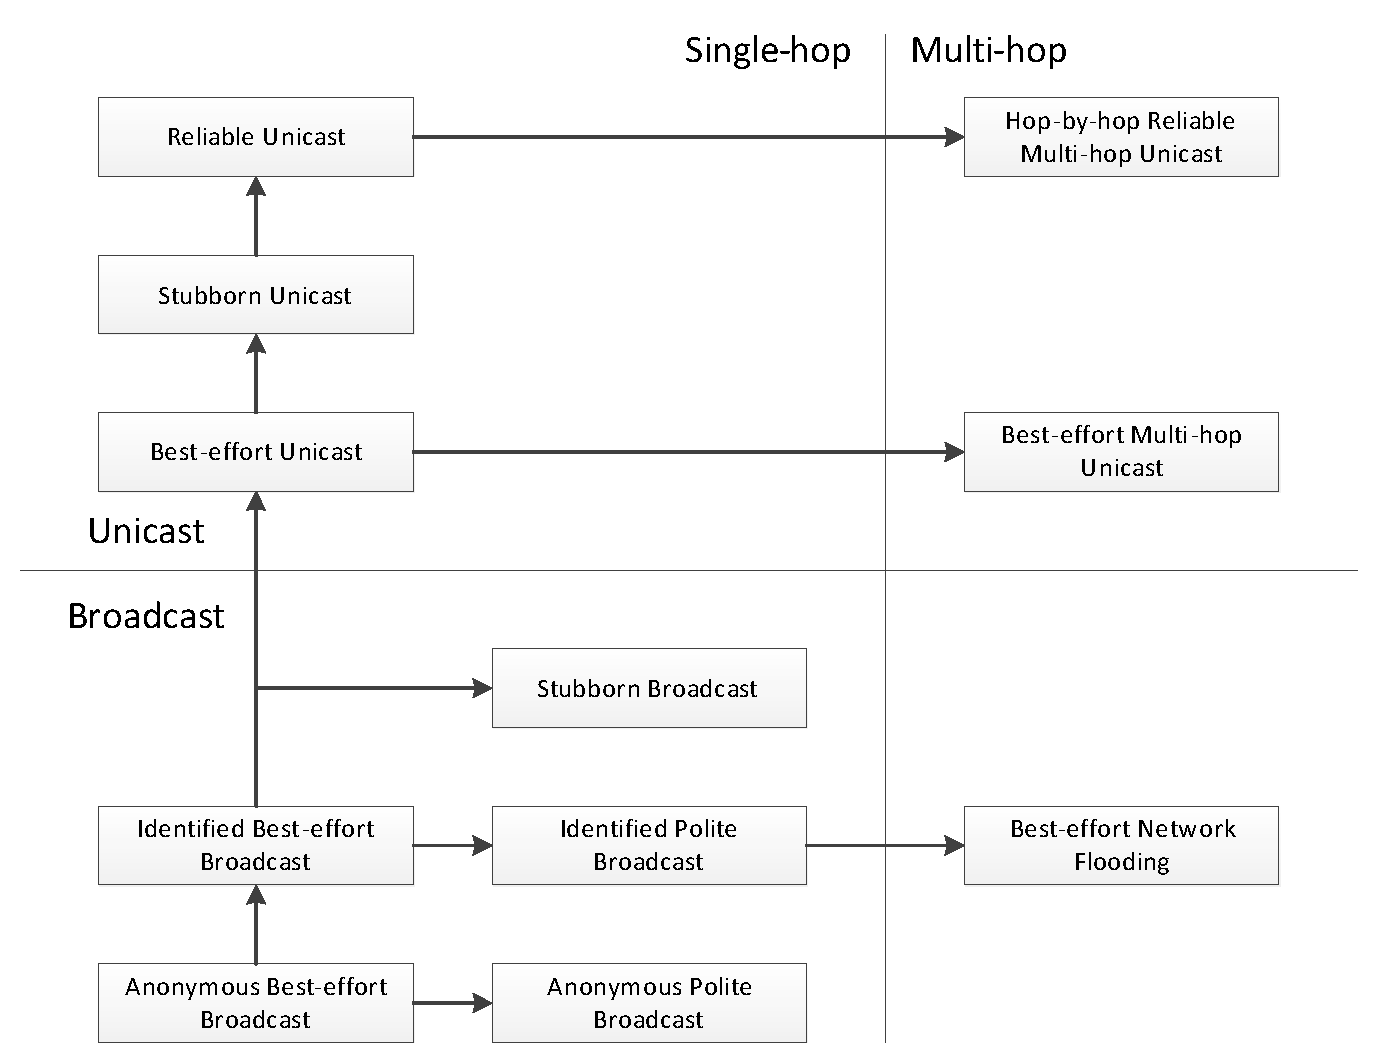
\includegraphics[width=0.8\textwidth]{Diagrams/rime-stack}
	\caption{The communication primitives in the Rime network stack \cite{Dunkels:2007:ACA:1322263.1322295}}
\end{figure}

\begin{table}[H]
	\centering
	\begin{tabular}{ | l | l | l | }
		\hline
		Name & Header & Address \\
		\hline
		Anonymous Broadcast & abc.h & \url{http://contiki.sf.net/docs/2.6/a01717.html} \\
		Broadcast & broadcast.h & \url{http://contiki.sf.net/docs/2.6/a01720.html} \\
		Stubborn Broadcast & stbroadcast.h & \url{http://contiki.sf.net/docs/2.6/a01739.html} \\
		Anonymous Polite Broadcast & polite.h & \url{http://contiki.sf.net/docs/2.6/a01730.html} \\
		Polite Broadcast & ipolite.h & \url{http://contiki.sf.net/docs/2.6/a01724.html} \\
		Unicast & unicast.h & \url{http://contiki.sf.net/docs/2.6/a01738.html} \\
		Stubborn Unicast & stunicast.h & \url{http://contiki.sf.net/docs/2.6/a01740.html} \\
		Reliable Unicast & runicast.h & \url{http://contiki.sf.net/docs/2.6/a01738.html} \\
		Network Flooding & netflood.h & \url{http://contiki.sf.net/docs/2.6/a01728.html} \\
		Multi-hop Unicast & multihop.h & \url{http://contiki.sf.net/docs/2.6/a01726.html} \\
		Reliable Multi-hop Unicast & rmh.h & \url{http://contiki.sf.net/docs/2.6/a01732.html} \\
		Reliable Unicast Bulk Transfer & rucb.h& \url{http://contiki.sf.net/docs/2.6/a00365.html} \\
		\hline
		\hline
		Mesh & mesh.h & \url{http://contiki.sf.net/docs/2.6/a01725.html} \\
		Collect & collect.h & \url{http://contiki.sf.net/docs/2.6/a01723.html} \\
		Trickle & trickle.h & \url{http://contiki.sf.net/docs/2.6/a01742.html} \\
		\hline
	\end{tabular}
	\caption{Communication Primitives, headers, and documentation location}
\end{table}

\begin{table}[H]
	\centering
	\begin{tabular}{ | l | l | l | l | }
		\hline
		Name & Reliable & Target & Sender Known\\
		\hline
		Anonymous Broadcast & No & 1-hop neighbours & No\\
		Broadcast & No & 1-hop neighbours & Yes\\
		Stubborn Broadcast & No & 1-hop neighbours & No\\
		Anonymous Polite Broadcast & No & 1-hop neighbours & No\\
		Polite Broadcast & No & 1-hop neighbours & Yes\\
		Unicast & No & destination & Yes\\
		Stubborn Unicast & No & destination & Yes\\
		Reliable Unicast & Yes & destination & Yes\\
		Network Flooding & No & network & Yes\\
		Multi-hop Unicast & No & destination & Yes\\
		Reliable Multi-hop Unicast & Yes & destination & Yes\\
		\hline
		\hline
		Mesh & No & destination & Yes \\
		Collect & Yes & destination & Yes \\
		Trickle & Yes & network & No \\
		\hline
	\end{tabular}
	\caption{Communication Primitives behaviour}
\end{table}

\paragraph{Flooding and Gossiping} Flooding and Gossiping are arguably the most simplistic routing algorithms available to a wireless sensor network developer. In flooding, wireless sensor network nodes broadcast to all their neighbours any messages that they receive, messages only stop when either i) the packet arrives at its intended recipient or ii) the messages maximum number of node hops is reached. Gossiping is similar to flooding in many ways, the only difference being that when a node receives a message, instead of broadcasting it to every neighbour, the node randomly picks one neighbour to forward the message to. Due to the simplicity of Flooding and Gossiping there is no need for any complex routing algorithms or topology maintenance \cite{Akkaya2005325}. However, these two routing algorithms do suffer from several drawbacks, these are: \emph{Implosion} -- is when the same message is sent to the same recipient twice (Gossiping avoids this but causes delays in the propagation of messages through the network), \emph{Overlap} -- is when two nodes sense the same change in a local environment and both send similar messages to the same neighbour and \emph{Resource Blindness} --  is when the routing algorithm consumes large amounts of energy with no consideration for efficiency \cite{Akkaya2005325}. Sensor Protocols for Information via Negotiation (SPIN) is a family of routing algorithms designed to address the issues with traditional Flooding and Gossiping protocols\cite{TankBible, Akkaya2005325}. The family does this by using data negotiation and resource-adaptive algorithms, for example nodes running SPIN have access to the their current battery level and use this information to adapt the protocol based on how much energy is remaining. Additionally, the SPIN family of protocols uses the concept of meta-data to reduce the level of redundant data sent around the network.

\paragraph{Clustering} Clustering is a form of hierarchical routing that has a long history of improving the efficiency of networks, originally being used to find the optimal placement of logic gates in digital circuits \cite{clustering}. In both these early applications and more modern variations the basic principle of clustering remains the same; to group (in a logical sense) nodes of a network according to their (typically geographic) locality \cite{1628365}. Each node in one of these \emph{clusters} has a single point of contact with the rest of the network, in a wireless sensor network this is a specific node in each cluster known as the cluster head (CH). Cluster heads communicate with each other and the base station to route packets around the network. The benefit of clustering a network is in reducing global network traffic, in a clustered network each node need only route messages to its CH rather than all the way to its destination. In some applications the CH can perform data aggregation or use a compression function\cite{1285913, aggregation} on the messages it forwards to reduce traffic between clusters; the nature of these functions is always application-specific. However, the nature of clustering means that a cluster head has a significantly higher workload than any other node in its cluster, as it must listen to every message sent from the cluster and possibly forward just as many messages to the other cluster heads in the network. In domains where nodes do not have a permanent power source (such as WSNs), this leads to greater energy usage in CHs, causing their batteries to drain faster\cite{placement}. As a result of this, many modern clustering algorithms (e.g. \cite{eemc, secc}) rely on or take inspiration from the Low Energy Adaptive Clustering Hierarchy (LEACH) \cite{LEACH}.

LEACH and LEACH-C are two clustering algorithms proposed by \citeauthor{LEACH}, in their paper the authors showed that the standard LEACH protocol performed significantly better than static clustering in terms of energy efficiency, with LEACH-C performing better still. However, the inclusion of both rounds and TDMA in LEACH means that it requires nodes in a WSN to be synchronised, which comes with significant implications in terms of operational complexity. LEACH itself offers no solutions either towards ensuring that nodes maintain synchronisation, or towards detecting if some nodes (or more likely, an entire cluster) is not performing correctly due to slipping from the prescribed TDMA schedule. However, the authors themselves suggest that a possible improvement to negate the need for TDMA is some event-based method for applications in which nodes do not generate transmissible data constantly or at prescribed intervals.

\paragraph{Tree Aggregation} Tree aggregation is another hierarchical routing protocol, which differs from clustering in that it divides a network into a tree structure with the root node situated at the base station. Nodes that are furthest from the base station (in hops) become leaves of the tree and any intermediate nodes become branches. Leaves and branches forward messages towards the base station and around the network using the tree structure, this results in a reduced number of global network messages over other algorithms such as flooding. The message count can be further reduced in a similar way to clustering, by implementing an aggregation or compression function at each branch node of the network. The drawbacks of tree aggregation are clearly similar to clustering: i) branch nodes have a higher workload than leaf nodes ii) if a branch node's battery is depleted and the node turns off it can disconnect an entire section of the network from the base station. There are several prominent tree aggregation algorithms (such as TAG, MFS and DCTC \cite{1628365}). Although very similar, they all take differing approaches to organising the data aggregation process of the branch nodes in order to reduce the number of collisions -- and therefore messages -- in the network. For example, TAG uses the idea of a periodic traffic pattern which is divided into time intervals for each layer of the tree, which ensures that each branch receives as many messages from its children as possible before it forwards to the next layer.   

\subsection{Summary}
In summation, we have explored many issues related to the field of wireless sensor networks with a specific focus on debugging them. Firstly, we examined the types of predicates our system might be required to check for, we aim to cover all 6 types of predicates, these are: strong, weak, stable, unstable, global and local. We also discussed the fault-error-failure cycle, with consideration to its impact on predicate language development. We decided upon attempting to detect error states and failures instead of faults, as these are best suited for a predicate language to detect. Next, we considered existing predicate checking software. We looked at 5 algorithms: H-Send, Sympathy, DIKON, DIDUCE and NodeMD. We compared and contrasted each algorithm and found that H-Send was the closest to our proposed system, in terms of its approach of defining a predicate. However, they were all very practically-oriented implementations as opposed to our proposed system which traces its roots from theoretical work in global predicate detection. We also considered the various platforms that are available to developers of programs for wireless sensor networks. JProwler is a Java implemented simulation of MICA motes, although it allows for fast implementation and rapid prototyping, code would then to be rewritten to work on a real wireless sensor network. NS2 is another network simulator with a focus on wired networks, meaning that it was unsuitable for our purposes. TinyOS is a complete operating system for wireless sensor nodes, in which programs are written in nesC, a dialect of C. TOSSIM is a simulator designed to run TinyOS programs and the whole system is event-driven. The alternative to TinyOS is Contiki, an open source event driven operating system for wireless sensor nodes, using the standard C language (with a range of libraries). Cooja is a simulator for the Contiki OS and provides plenty of tools for developers such as a network visualiser and network communication log. We then looked at some current practical applications of wireless sensor networks, this showcased what wireless sensor technology is used for and more importantly what users of the technology might require from our system. The breadth of real-world applications was staggering, from volcano to animal habitat monitoring and everything in between. Finally, we discussed the several traditional types of routing algorithms available for distributed systems (e.g. flooding, clustering and tree aggregation). We then looked at several algorithms designed specifically for wireless sensor networks (e.g. SPIN, LEACH and TAG), we discussed the improvements made and what benefits they brought to the traditional algorithms.